% !TEX program = arara-rc
% !TEX encoding = utf8
% !TEX spellcheck = en_GB
%:!arara settings
% arara: lualatex: { shell: true , synctex: true }
% !arara: lualatex: { shell: true , synctex: true }
%%: Start Header
\makeatletter
\RequirePackage{ifluatex}
\ifluatex
 \else
   \PackageError{xframed}{
    ^^J\space\space * This file requires LuaTeX.       
    ^^J\space\space * You  must change your typesetting engine                
  }
  \expandafter\endinput
\fi
\makeatother
\setcounter{errorcontextlines}{999}
\documentclass[openany,12pt,tocdepth=3]{ltx-md}
\usepackage{xframed}
\usepackage{frcursive}
\usetikzlibrary{decorations.pathmorphing}
\RequirePackage{minted}
\usemintedstyle{autumn}
\fvset{xleftmargin=0.2cm,xrightmargin=.2cm}
\renewcommand*{\dictumwidth}{.5\textwidth}
\setcounter{secnumdepth}{3}

\ExplSyntaxOn
\keys_define:nn {ltxexample}
 {
  caption  .tl_set:N = \l_mdxex_caption_tl,
  label    .tl_set:N = \l_mdxex_label_tl,
  minted   .tl_set:N = \l_mdxex_minted_tl,
  minted   .initial:n = {linenos=true} ,
  language .tl_set:N = \l_mdxex_language_tl,
  language .initial:n = latex,
  result   .bool_set:N = \l_mdxex_result_bool,
  result   .initial:n =false,
 xframed .tl_set:N = \l_mdxex_xframed_tl,
}

\NewDocumentEnvironment {ltxexample} { O {} }
 {
  \keys_set:nn { ltxexample }
   {
    #1
   }
  \group_begin:
  \tl_set:Nx \l__mdxex_temp_tl
   {
    \exp_not:N \VerbatimEnvironment
    \tl_if_empty:NTF \l_mdxex_caption_tl
     {
      \scan_stop:
     }
     {
      \exp_not:N \xframedsetup 
          {
             line-color=brown!70!black,
             bg-color=brown!10!white,
             inner-top-margin=12pt,
             inner-bottom-margin=6pt,
             title-skip-above = 6pt,title-skip-below=6pt,
             title-bg-color = brown!15!white,
             line-width-top=2pt,margin=1cm,
             first-title= { \exp_not:N \captionof { lstlisting }{ \exp_not:V \l_mdxex_caption_tl } 
                                \tl_if_empty:NF \l_mdxex_label_tl
                                 { \exp_not:N \label { lst\exp_not:N : \l_mdxex_label_tl } }
                               } 
         }
     }
    \exp_not:n { \begin{xframed}}
      [ \exp_not:V \l_mdxex_xframed_tl ]
    \exp_not:n { \begin{minted} } [ \l_mdxex_minted_tl ] { \l_mdxex_language_tl }
   }
  \l__mdxex_temp_tl
 }
 {\end{minted}\end{xframed}%
  \group_end:\bool_if:NT \l_mdxex_result_bool { \input{\jobname.pyg} }
}

\RenewDocumentCommand\DeleteFile{m}{}
\Newxframedenv
 [
  line-color=green!60!black,
  bg-color=green!10,
  head = { \textcolor{green!60!black}{ \faInfoSign } },
 ]{Note}
\ExplSyntaxOff
\NewDocumentCommand \Github {} {Github\faGithub\xspace }
\def\theFancyVerbLine{\rlap{\rmfamily\tiny\arabic{FancyVerbLine}}}
\begin{document}
\title{The \Pack{xframed} package}
\subtitle{This is an alpha-version}
\author{Marco Daniel}
\date{\today}
\notes{As shown in the subtitle this is an alpha version. Use this package on your own
risk.\\[.5cm]
I know my English is really poor and the quality of the documentation suffers on it. 
So I am really happy about any improvments.\\[1cm]

As long as the package has the version alpha I am not deprecated to change names
of options. My aim is to use as many intuitive options as possible. 
}
\maketitle
\vspace*{\fill}
\begin{xframed}[line-width=3pt,line-color=purple!30!white,bg-color=yellow!10,developer-info,margin=1cm]
\rule{0pt}{5cm}
\end{xframed}
\clearpage
\pdfbookmark[1]{\contentsname}{tocbook}
\tableofcontents


\setchapterpreamble[o]{\dictum[\href{http://tex.stackexchange.com/a/18360/5239}{Gonzalo Medina at TeX.SX}]{%
Expand $(a+b)^n$:
\begin{center}
  \count255=0
  \loop\advance\count255 by 10
  \ifnum\count255<40
    $(a\hskip\count255 pt +\hskip\count255 pt b)^n$\\
  \repeat
\end{center}}}
\addchap{Preface}
\addsec{Introduction}\label{sec:intro}
I am interested in \LaTeX\ and specially in \LaTeX3. With this package I want
to improve my skills using this great language. However I am a beginner and
so the package has only an \textit{alpha} version. If you use this package
be aware of this situation. I am sure the great guys at
\faArrowRight\href{http://tex.stackexchange.com/}{TeX.SX} will help me to improve this package.


\addsec{Bug reports}\label{sec:bug-reports}
Bug reports can be done at
\href{https://github.com/marcodaniel/xframed/issues}{xframed at \Github}. If you have no
account at \Github you can drop me an e-mail
\href{mailto:marco.daniel@mada-nada.de}{\faEnvelope marco.daniel@mada-nada.de}

\addsec{Installation}
As long as the package isn't available at CTAN you must install (if you dare it)
manual. Therefor you can clone the repository in your local texmf tree. I provided
the correct folder structure at \Github to simplify the installation.

\setchapterpreamble[o]{\dictum[]{%
If you are only interested in the usage of the package you can
skip this chapter. All options are explain in \autoref{chap:usage}}}
\chapter{Idea behind \texorpdfstring{\Pack{xframed}}{xframed}}\label{chap:idea}

The idea is very simple. Draw a frame around given material. During my study 
I wanted a package which can be break across pages and put a frame around this.
The package \Pack{framed}\footnote{Package \Pack{framed} by Don­ald Arse­neau, 
see \href{http://www.ctan.org/pkg/framed}{CTAN: framed}} didn't require my needs.
So I started to write my own package. The result can be found at CTAN, too. It's the
package \Pack{mdframed}\footnote{Package \Pack{mdframed} by Marco Daniel, 
see \href{http://www.ctan.org/pkg/mdframed}{CTAN: mdframed}}.

After passing my study I started to improve the package \Pack{mdframed}. In 2011 
I registered at \href{http://tex.stackexchange.com/}{TeX.SX}  and learned something
about the new language \Pack{expl3}\footnote{see: 
\href{http://latex-project.org/latex3.html}{http://latex-project.org/latex3.html}}. 
I was so fascinated about the great work of the \LaTeX3 core team that I started 
my first steps with simple functions. I also wrote a small article about the 
frontend \Pack{xparse} for the German community. The article was published
in   \emph{Die \TeX nische Komödie 2/2012}. 
After a while I wanted to provide my own \Pack{expl3}-package. Now here it is.

I know most users love examples. So I am trying to provide a lot. All
frames in this documentation are done by \Env{xframed}. So I hope
you will have some inspiration. The highlight of listings is done
by \Pack{minted}\footnote{Package \Pack{minted} by Kon­rad Ru­dolph, 
see \href{http://www.ctan.org/pkg/minted}{CTAN: minted}, now maintained by G. Poore.}.

\vfill
By the way. The compilation of this document is done with the
typesetting engine \LuaLaTeX. To simplify my compilation steps
I am using the cool tool \Pack{arara}\footnote{Tool \Pack{arara} by Paulo Cereda, 
see \href{http://www.ctan.org/pkg/arara}{CTAN: arara}}.

\vfill
Now it's time to introduce the package.


\setchapterpreamble[o]{\dictum[\href{http://tex.stackexchange.com/a/18370/5239}{Jaime Soto at TeX.SX}]{%
\begin{eqnarray*}
    \begin{bmatrix}
    \cos 90^{\circ} & \sin 90^{\circ}\\
   -\sin 90^{\circ} & \cos 90^{\circ}
\end{bmatrix}
\begin{bmatrix} a1 \\ a2 \end{bmatrix}
=
\rotatebox[origin=c]{270}{$\begin{bmatrix} a1 \\ a2 \end{bmatrix}$}
\end{eqnarray*}}}
\chapter{Usage}\label{chap:usage}
The following sections describe the options of the package and the provided 
environments. The basic environment is equal to the package name \Env{xframed}.

\section{Loading the package}
Before you can use the package, you must load it in your preamble. As usual the 
package is loaded by \Cmd{usepackage}. The following listings shows it.
\begin{ltxexample}[caption=Loading the package,label=loading]
 % Preamble
 \usepackage{xframed}
\end{ltxexample}
If you have done this you can use the basic environment \Env{xframed}.

\ExplEnv{xframed}
The environment has one optional argument where you can specify options
which are only used for this frame. The following listings demonstrates the usage.
\begin{ltxexample}[caption=Loading the package,label=loading]
 % document body
 \begin{xframed}[option-list]
   The contents of the frame
 \end{xframed}
\end{ltxexample}

\section{Specifying the options}\label{sec:specopt}
Before you setup any options you must understand hot the frame is drawn.
The default method is by using \Pack{TikZ}\footnote{Package \Pack{TikZ} by 
Till Tantau \& friends, see \href{http://www.ctan.org/pkg/pgf}{CTAN: TikZ}}. 
\Pack{TikZ} allows a very user friendly way to setup high quality graphics. 
Therefor all elements are specified by \Pack{TikZ} options. The basic command
to manipulate these elements is \Cmd{xframedsetuptikz}. The usage is explained
in \autoref{se:tikzsetup}.  All other options can be set by \Cmd{xframedsetup}. 
Both command can be used in the preamble or inside the document body. If
you enclose these commands inside a group the settings will be local, too.
 
\ExplCmd{xframedsetuptikz\MArgs}
The command has one mandatory argument. The mandatory argument accepts only
defined options which are explained in \autoref{se:tikzsetup}

All other options can be setup by the command \Cmd{xframedsetup}.
\ExplCmd{xframedsetup\MArgs}
This command has one mandatory argument. All allowed options are explained
in \autoref{chap:options}. 

\ExplCmd{newxframedstyle}[\MArgs[style-name]\MArgs]
Often it is useful to declare a style with the needed options. Therefor
you can use the command \Cmd{newxframedstyle}. The command
has two mandatory arguments. The first mandatory argument
is the name of the style. Internal the style name is saved
as \verb+xframed_style_<style-name>_user+. That means normally
you can use every style name without any risk. If the style already exists
\Pack{xframed} uses the commmand \Cmd{renewxframedstyle} and
provides a warning.

After you have defined a style you can use the name of the style as
a legal value of the option \Opt{style}.

\ExplCmd{renewxframedstyle}[\MArgs[style-name]\MArgs]
If you wan to redefine an existing style you can do this by 
\Cmd{renewxframedstyle}. The syntax of the command
is equal to \Cmd{newxframedstyle}. If the style doesn't exist
\Pack{xframed} uses the command \Cmd{newxframedstyle} and
provides a warning.

\ExplCmd{addtoxframedstyle}[\MArgs[style-name]\MArgs]
If you want to extend a predefined style you can do this
with \Cmd{addtoxframedstyle}. The command has the same
syntax as \Cmd{newxframedstyle}. If the style doesn't exist
\Pack{xframed} uses the command \Cmd{newxframedstyle} and
provides a warning.

\ExplOpt{style}
The option \Opt{style} needs the name of a predefined style
by \Cmd{newxframedstyle} . All options declared with \Cmd{newxframedstyle} 
will be used.


\section{Helper functions}\label{sec:helperfunctions}
The next function will normally be used by advanced users. However
I decided to put this information here instead of in
\autoref{chap:developer-info}~\nameref{chap:developer-info}.
All commands have one mandatory argument. The mandatory argument
is one of the explained keys in the following sections. 

\begin{Note}
The mandatory argument of any helper function doesn't accept a meta key.
\end{Note}

\ExplCmd{usexframendlength}[\MArgs[key]]
This command  allows you to use the
provided length inside an other command. The \texttt{key} is one of
the length keys explained in the following sections. 
\ExplCmd{showxframendlength}[\MArgs[key]]
The command \Cmd{showxframendlength} has one important
difference to \Cmd{usexframendlength}. The provided length
can be printed inside the document. For you my \TeX-hacker
that means the primitive \Cmd{the} is used. 

\ExplCmd{usexframendskip}[\MArgs[key]]
This command is equal to \Cmd{usexframendlength} whereby
a skip key is required.
\ExplCmd{showxframendskip}[\MArgs[key]]
I think you know what happen here. See \Cmd{showxframendlength}, 
it's only for skip length.
\ExplCmd{usexframendcolor}[\MArgs[key]]
This command is similar to the command \Cmd{color}, whereby the
color of the provided option is used.
\ExplCmd{showxframendcolor}[\MArgs[key]]
This command print out the color which is hidden under the key.

\minisec{Example}
Next to the explanation I want to provide an example. 

\begin{ltxexample}[caption=Example of helper functions,label=helper,result=true,]
 \begin{xframed}[margin=3cm]
    \centering
    \xframedsetup{inner-margin-left=1cm}
    \showxframendskip{skip-above}%
    \rule{\usexframendlength{inner-margin-left}}{2pt}%
    \showxframendcolor{font-color}
 \end{xframed}
\end{ltxexample}


\section{Creating new environments}\label{sec:newenv}

As explained above the package \Pack{xframed} provides
one basis environment \Env{xframed}. To provide new
environments which use \Env{xframed} you can work with
the normal \LaTeXe command \Cmd{newenvironment} or
the command \Cmd{NewDocumentEnvironment} provided
by \Pack{xparse}. However \Pack{xframed} tries to simplify
the process by the following commands.

\ExplCmd{Newxframedenv}[\OArgs\MArgs[env-name]]
Create a new environment with the name of the mandatory argument
of \Env{Newxframedenv}. The optional argument accepts all
defined keys of \Pack{xframed}.

\ExplCmd{Renewxframedenv}[\OArgs[env-name]]
This command is similar to \Cmd{Newxframedenv} whereby
the command must already exist.

\ExplCmd{Surroundwithxframed}[\OArgs\MArgs[env-name]]
Sometimes you have predefined environments like \Env{verbatim}
where you want to get a colored background. To do this you can 
surround existing environments with \Cmd{Surroundwithxframed}
where the mandatory argument is the name of the existing environment.
The optional argument accepts all keys defined by \Pack{xframed}.
\begin{Note}
The declaration by \Cmd{Surroundwithxframed} works global.
\end{Note}

Before we start with options we need to understand the provided elements of the frame. 

\section{Elements of the frame drawn by \texorpdfstring{\Pack{xframed}}{xframed}}
It should be clear the a frame has some rules around. So we can check mark the first
relevant point.The next point of the agenda is the main body, the title and the foot. These
three elements are very important to understand the behavior. The simple picture below
should show the elements and the provided names inside the package.

\begin{center}
\captionof{figure}{Base elements of \texorpdfstring{\Pack{xframed}}{xframed}}\label{fig:baseelements}
\begin{tikzpicture}[outer sep=0pt]
 \node[draw,fill=gray!20,rectangle,minimum width=8cm, minimum height=2cm,font=\bfseries] (main) {Body of the frame~\faArrowRight~\texttt{main}};
 \node[draw,fill=gray!30,rectangle,minimum width=8cm, minimum height=1cm,font=\bfseries,anchor=south] at (main.north) {Title of the frame~\faArrowRight~\texttt{first-title}};
 \node[draw,fill=gray!30,rectangle,minimum width=8cm, minimum height=1cm,font=\bfseries,anchor=north] at (main.south) {Foot of the frame~\faArrowRight~\texttt{last-foot}};
\end{tikzpicture}
\end{center}
I know the picture looks very poor at the beginning but we want to concentrate on the
main issue. It describes the three base elements of the frame drawn by \Env{xframed}.

\vspace*{\baselineskip}
Now let's start with all options. Be aware the list ist long. 

\setchapterpreamble[o]{\dictum[\href{http://tex.stackexchange.com/a/18354/5239}{Paulo Cereda at TeX.SX}]{%
Find $x$.

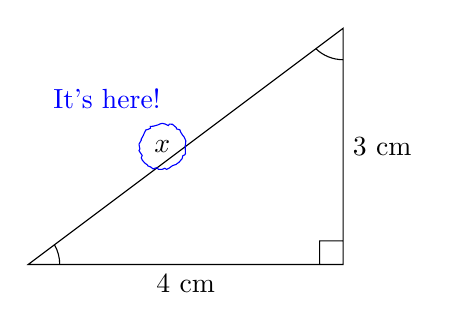
\begin{tikzpicture}
\draw (0,0) -- (4,0) node[midway,below] {4 cm}
   -- (4,3) node[midway,right] {3 cm}
   -- (0,0) node[midway,left,circle,draw=blue,decorate,decoration={random steps,segment length=1pt,amplitude=0.5pt}]{$x$}
   -- (4,0) rectangle (3.7,0.3)
   -- cycle;
\draw (0.4,0) arc (0:30:0.5);
\draw (4,2.6) arc (270:226:0.5);
\draw (1,2.1) node []{\color{blue}\fontfamily{frc}\selectfont{It's here!}};
\end{tikzpicture}}}

\chapter{Package options}\label{chap:options}
Every user has his/her own wishes. It's very difficult to implement an evironment 
which meets all requirements. I hope with the following options you can setup your 
requirements as best as I was able to implement. As described in \autoref{chap:idea}
the package uses \Pack{expl3} in the background. So I can provide more intuitive names.
During the explanation I refer to the environment \Env{framed}. However this is only
symbolic. The options are also working for other derivations. 

\Pack{xframed} provides some meta keys. That means if you pass a value
to the meta option more than one other option are influenced. Every meta
option has a star~{\let\quad\relax\Metakey}~right of the name. 

\section{Drawing method}\label{sec:method}

As \Pack{mdframed} I decided to support different methods of frame drawing.

The usage of TikZ or PSTricks needs a lot more compilation time then the normal
\LaTeX\ command \Cmd{rule}. In most cases a simple \Cmd{rule} is ok. However
instead of \Pack{mdframed} you can choose the method for every frame separate.

\begin{Note}
Up to know there is no PSTricks implementation.
\end{Note}

\ExplOpt[tikz]{frame-method}
The option \Opt{frame-method} allows you to declare the drawing commands.
All allowed options are:
\begin{center}
\def\arraystretch{1.25}
\begin{tabular}{@{}>{\MacroFont}lp{0.6\linewidth}@{}}\hline
 default, tex, latex, none& Draw the frame with standard \LaTeXe commands. It needs the least compilation time.\\
 pgf, tikz& Draw the frame with TikZ. It needed the highest compilation time.\\
 pstricks, ps , postscript& Draw the frame with PSTricks.  \\\hline
\end{tabular}
\end{center}

\ExplOpt{tikz*,default*}
These options aren't meta option but I want to emphasize them. Theses options are 
short forms of \Opt{frame-method}\texttt{=tikz} respectively \Opt{frame-method}\texttt{=default}.
The options don't allow any values.


\section{Outside the frame}
Drawing a frame requires some modifications around. So you want to setup the margins
or the skips above or below the frame. Related to the meaning of the keys, all keys 
requiers a length or skip dimension. That mean that the length variables defined as
\texttt{dim} have a fixed length, whereas \texttt{skip} length can have a rubber (stretch/shrink) component. 

\ExplOpt[\string\linewidth]{width}
This key allows you to specify the width of the complete frame. 
Normally you don't need this key. All related length (left margin, right margin)
can be specified by options. 


\ExplOpt[10\,pt]{skip*,skip-above,skip-below}
The lengths represent the space before and after the environment \Env{xframed}.  
This option \Opt{skip} is a meta key and sets the \Opt{skip-below} and \Opt{skip-above} to the given skip length. 


\ExplOpt[0\,pt]{margin*,margin-left,margin-right}
Normally the frame \Env{xframed} is drawn about the complete text width. However this isn't
often very common shrinking the outer margin. This keys accept a dimension length 
which specify the left and the right margin. You can also use negative values. In this case the frame 
is drawn inside the margin of the page.


\ExplOpt[0\,pt]{extra-skip}
Sometimes it's useful to add some vertical white space in front of the frame. This can be useful
if you want some elements on the lines. To take care of this required space you can
set the Option \Opt{extra-skip}. Negative dimensions are also allowed whereby I can't
image any situation to use it. 



\vspace*{\baselineskip}
This finished the \emph{outside} part for the moment. The package provides also some hooks
which will can be used as an option. This isn't really a low level issue so these
options are described in \autoref{sec:hook}. 

\vspace*{\baselineskip}
Before I will describe the options related to there base element as shown in \autoref{fig:baseelements}, 
I will start with the rules around the frame.

\section{Rules around the frame}\label{sec:lines}
A normal frame has four sides. The frame of \Env{xframed} isn't an exception. Of course
you can manipulate as possible to get a triangle or a star.

\ExplOpt[0.8\,pt]{line-width*,line-width-left,line-width-right,line-width-top,line-width-bottom}
The first option in this section specify the width of all four lines around the material of \Env{xframed}.
This implies the title and the foot of the frame. If you want to setup the rule width of the elements
separate you can do this by the following options.


The width is only one part of the lines. I am sure you want to change the colors too. 
\ExplOpt[black]{line-color*,line-color-right,line-color-top,line-color-bottom}
Normally all lines have the same color. The color for all four lines can be specified 
with the Option \Opt{line-color}. However the following keys allow the color
specification separate.


\minisec{Example}
I think it's time for a small example. Suppose you want that all lines has a width of
2\,pt expect the top line which shall have a width of 4pt and a different color.
This can be achieved by
\begin{ltxexample}[caption=Example outer part,label=outer,result=true,]
 \begin{xframed}[line-width=2pt,line-width-top=4pt,
          line-color-top=blue]
   The contents of the frame
 \end{xframed}
\end{ltxexample}
As a small revision we can achieve the same effect with \Cmd{xframedsetup}, 
whereby the settings are used for the the environments \Env{xframed} to follow.
\begin{ltxexample}[caption={Example outer part II},]
 \xframedsetup[line-width=2pt,line-width-top=4pt
           ,line-color-top=blue]
 \begin{xframed}
   The contents of the frame
 \end{xframed}
\end{ltxexample}

As you can see the topline gets a smooth transition. 

\ExplOpt{show-all-lines*}%metakeys
By default a frame has four lines around it. Drawing no
lines can be achieved by the boolean flag \Opt{show-all-lines}.
If you don't want to draw any lines you can pass the value \texttt{false}
to the option \Opt{show-all-lines}

\ExplOpt[true]{top-line,left-line,bottom-line,right-line}%bool-option
The option \Opt{show-all-lines} controls the behavior
of all lines. But you can control every line separate. The option 
\Opt{top-line} and friend influence the lines of the frame. All four are 
boolean keys and accepts either \texttt{true} or \texttt{false}.


\ExplOpt[10\,pt]{round-corner*,arc*,arc-outer,arc-inner}
The arc of the corners can be controlled by the provided keys. Thereby
you can manipulate the outer arc and the inner arc separate.
I provided two meta keys because I couldn't provide a correct name.
That means the value of \Opt{round-corner} or \Opt{arc} is passed
to the options \Opt{arc-outer} and \Opt{arc-inner}. 

\minisec{Example}
I think it's time for a small example.

\begin{ltxexample}[caption=Example outer part III,result=true,label=arc]
\newxframedstyle{example-outerpart}
   { line-width=4pt,margin=1cm,line-color=red!40!black,
     bg-color=red!20,round-corner=20pt,arc-outer=5pt}
\begin{xframed}[style=example-outerpart]
 \begin{minted}{latex}
   \newxframedstyle{example-outerpart}
     { line-width=4pt,margin=1cm,line-color=red!40!black,
       bg-color=red!20,round-corner=20pt,arc-outer=5pt}
 \end{minted}
 The contents of the frame with some text
 and some more text. And more text.
\end{xframed}
\end{ltxexample}

\section{Main body of the frame}\label{sec:element-main}
As shown in \autoref{fig:baseelements} the body is the main part of
the environment \Env{xframed}. Inside the body you can use every
material also verbatim one. This part is save in a single coffin%
\footnote{See: \Pack{l3coffin}}  and allows such things. 

\ExplOpt[\string\normalfont]{font}
The option \Opt{font} allows the specification of the main part of \Env{xframed}.
It doesn't influence the other part. 

\ExplOpt[black]{font-color}
If you want to change the font color you can do this with the option \Opt{font-color}.

\ExplOpt[white]{bg-color}
The complete background of \Env{xframed} is specified by the color given
as an argument of \Opt{bg-color}. If you want some shadings or whatever
you can imagine you can the power of TikZ. How to do this
is explained in \autoref{sec:tikzsetup}.

\ExplOpt[10\,pt]{inner-margin*,inner-margin-left,inner-margin-right}
The distance on the left site and the right site of the frame will be 
controlled by \Opt{inner-margin-left} and \Opt{inner-margin-right}. The 
key \Opt{inner-margin} pass the value to the relevant lengths. 

\begin{Note}
The length will be used for the other two elements as shown in 
\autoref{fig:baseelements}, too.
\end{Note}

 Related to the left and right margin you can set the top and bottom margin.
\ExplOpt{inner-top-margin}
This keys sets the top margin of the main part.
\ExplOpt{inner-bottom-margin}
This keys sets the bottom margin of the main part.


\minisec{Head of the frame}
Sometimes you want to have a small head without any break. This
can be achieved by the key \Opt{head}. I implement this key with 
some other options to simplify e.g. the creating of a new theorem. There
is also another option \Opt{first-title} which is used in a new coffin and
so put in an extra box. At the moment all captions of the provided listings
are done in the \Opt{first-title}. 


\ExplOpt{head}
Puts the given argument of \Opt{head} at the beginning
of the main body.
\ExplOpt[\string\normalfont\string\sffamily\string\bfseries]{head-font}
The font is specified by the option \Opt{head-font} which be set set local as
also the color.
\ExplOpt[black]{head-font-color}
Specifies the color of the head.


\minisec{Head of the frame}
I guess at this point an example is useful. Instead of explaining I 
only provide the example.

\begin{ltxexample}[caption={Example main part},label=main,result=true]
 \begin{xframed}[%
   line-width=4pt,line-color=blue,
   inner-margin=1cm,font-color=blue!70,
   head={Example of Head},head-font-color={red!70},
   margin=1.5cm,bg-color=yellow!20,
  ]
   The contents of the frame and some filling text to 
  provide a second line.
 \end{xframed}
\end{ltxexample}


\section{Title of the frame}\label{sec:element-firsttitle}
The title of the frame is specified by an option and also save in a coffin. 
This means the paragraphs of the body can't be influence by material
of the title. Here you can see the first main differences between
\Opt{first-title} and \Opt{head}. Let us start with options.

\ExplOpt{first-title}
First of all we need a title. The title can be specified by \Opt{first-title}. The argument
is saved in a single token. Of course you can use line breaks but please en capsule
the whole argument in curly braces. Curly braces must be used if you argument contains
a comma. May you wonder why it's named \Opt{first-title}. If the frame
must be splitted the \Opt{first-title} is only used at the first frame. If
you don't have any splitted frame, you have only one tile the \Opt{first-title}.
\ExplOpt[\string\bfseries\string\sffamily\string\large]{title-font}
Normally the title should be highlighted. So I decided to declare the list of
font commands as default. However you can use the option \Opt{title-font} to
declare your own font settings.
\ExplOpt[black]{title-font-color}
As usual you can specify the color of the font. This is done by the option
\Opt{title-font-color}.

\ExplOpt[5pt]{title-skip*,title-skip-above,title-skip-below}
As written the title is put inside a new coffin. The explained options \Opt{inner-margin},
\Opt{inner-margin-left} and \Opt{inner-margin-right} will be used on the left and right side of
the title component. However you can specify the length above and below the contents of the title. 
The option \Opt{title-skip} passes the argument to the options \Opt{title-skip-above}
and \Opt{title-skip-below}.


\begin{Note}
I know the name \texttt{skip} leads to irritations. The length are saving in a
dimension register and so any glue  is cut off.
\end{Note}

\ExplOpt[white]{title-bg-color}
As the main part you can specify a different color as background for
the title. This color of the option \Opt{title-bg-color} will be used for it.


The package \Pack{xframed} provides a single line between the title and the main body.
The following options show you the usage. Of course with methods of
\autoref{sec:tikzsetup} you can draw dashed lines or other one as well.
\ExplOpt[true]{title-line}
The option \Opt{title-line} is a boolean key. If you say \texttt{true} a line to separate
the material will be drawn. If you say \texttt{false}, you will get no line.
\ExplOpt[0.6pt]{line-width-title}
The width of the line is specified by the option \Opt{line-width-title} whereby
the width doesn't influence the length \Opt{inner-top-margin} and \Opt{title-skip-below}.
\ExplOpt[black]{title-line-color}
Last but not least the color of the line is done by \Opt{title-line-color}.

\minisec{Example}
It's time for a new example to demonstrate the title.

\begin{ltxexample}[caption={Example title part},label=title,result=true]
 \begin{xframed}[title-bg-color=brown!30,%
   line-width=2pt,line-color=brown!60,
  first-title={This is the title of the frame},
   margin=1.5cm,bg-color=yellow!20, ]
   The contents of the frame and some filling text to 
  provide a second line.
 \end{xframed}
\end{ltxexample}



\section{Foot of the frame}\label{sec:element-lastfoot}
The settings of the foot element are equal to the title element. So 
the explanation will be short. 
\ExplOpt{last-foot}
The foot can be specified by \Opt{last-foot}. Of course now you
know why it is named \Opt{last-foot} (related to \Opt{first-title},
\ExplOpt[\string\bfseries\string\sffamily\string\small]{foot-font}
The foot is normally a little bit smaller so I decided to use \Cmd{small} as
default.


\ExplOpt[black]{foot-font-color}
Specify the color of the font.

\ExplOpt[5pt]{foot-skip*,foot-skip-above,foot-skip-below}
The option \Opt{foot-skip} passes the argument to the options \Opt{foot-skip-above}
and \Opt{foot-skip-below}. The distance between the separation line between the 
main part and the material of \Opt{last-foot} is controlled by \Opt{foot-skip-above}.
On the other hand \Opt{foot-skip-below} specifies
the length between the frame and the material of \Opt{last-foot}.

\begin{Note}
I know the name \texttt{skip} leads to irritations. The length are save in a
dimension register and so any glue will be cut.
\end{Note}

\ExplOpt[white]{foot-bg-color}
As the main part you can specify a different color as background for
the foot. This color of the option \Opt{title-bg-color} will be used for it.


The package \Pack{xframed} provides a single line between the foot and the main body.
The following options show you the usage. Of course with methods of
\autoref{sec:tikzsetup} you can draw dashed lines or other one as well.
\ExplOpt[true]{foot-line}
The option \Opt{foot-line} is a boolean key. If you say \texttt{true} a line to separate
the material will be drawn. If you say \texttt{false}, you will get no line.
\ExplOpt[0.6pt]{line-width-foot}
The width of the line is specified by the option \Opt{line-width-foot}.
\ExplOpt[black]{foot-line-color}
Last but not least the color of the line is done by \Opt{foot-line-color}.


\minisec{Example}
It's time for a new example to demonstrate the title.

\begin{ltxexample}[caption={Example foot part},label=foot,result=true]
 \begin{xframed}[title-bg-color=brown!30,%
   foot-bg-color=brown!30,line-width=2pt,
   line-color=brown!60,margin=1.5cm,bg-color=yellow!20, 
   first-title={This is the title of the frame},
   last-foot={you reached the end},]
   The contents of the frame and some filling text to 
  provide a second line.
 \end{xframed}
\end{ltxexample}


\section{Tikz elements of  \texorpdfstring{\Pack{xframed}}{xframed}}\label{sec:tikzsetup}
I often refer this section. The reason is very simple. \LaTeX without any 
extension can draw nice graphics. Therefor bundles like PSTricks
or TikZ/PGF are needen. This sections shows the implementation
using TikZ and so it allows a lot of modification. Please note this
documentation doesn't explain TikZ. Therefor you shall consolidate
the documentation of TikZ.

\ExplOpt{setup-tikz}%hooks--tl
The command to setup all TikZ styles was introduced in \autoref{sec:specopt}.
The needed command is \Cmd{xframedsetup}. Of course you can also use 
the option \Opt{setup-tikz} of \Env{xframed}. Nevertheless the syntax of
the implementation is equal, because the value of
\Opt{setup-tikz} is passed to \Cmd{xframedsetup}. 


\minisec{Excursus}
Let me do a small excursus. TikZ allows very simple to define
new styles by using the syntax of \Pack{pgfkeys}. For example
you wan to define your own style for some rectangles you can do this as follows.
\begin{ltxexample}[caption={Excursus TikZ style},label=excursus,result=false]
 \tikzset{my rectangle/.style={fill=green}}
 \tikz\draw[my rectangle] (0,0) rectangle (2,0.5);
\end{ltxexample}
The result will be \input{\jobname.pyg}. \Pack{xframed} does nearly the same.
Instead of using the family Tikz, \Pack{xframed} uses the family \texttt{xframed}.
That means every defined style has the prefix \texttt{xframed}. Related to our
example above \Pack{xframed} do:
\begin{ltxexample}[caption={Excursus TikZ style},label=excursusi,result=false]
 \xframedsetuptikz{my rectangle/.style={fill=green}}
 \tikz\draw[xframed/my rectangle](0,0) rectangle (2,0.5);
\end{ltxexample}
And you get the same result \input{\jobname.pyg}.\hfill {\small end excursus}


Next are all defined styles explained. You can change every style with the
syntax of TiKZ.  I hope I don't forget no element.

\ExplTOpt[fill = \Opt{bg-color}]{bg/.style}
This style controls the background of the main element. The
default is a full filled rectangle whereby the color
is specified by \Opt{bg-color}. 

\ExplTOpt[fill = \Opt{title-bg-color}]{title~bg/.style}
This style controls the background of the title element. The
default is a full filled rectangle whereby the color
is specified by \Opt{title-bg-color}. 

\ExplTOpt[draw = \Opt{title-line-color},line width\Opt{line-width-title}]{title~rule/.style}
This style controls the separation line between the main and the title element.

\ExplTOpt[fill = \Opt{foot-bg-color}]{foot~bg/.style}
This style controls the background of the foot element. The
default is a full filled rectangle whereby the color
is specified by \Opt{foot-bg-color}. 
\ExplTOpt[draw = \Opt{foot-line-color},line~width = \Opt{line-width-foot}]{foot~rule/.style}
This style controls the separation line between the foot and the title element.

\ExplTOpt[rounded~corners = \Opt{arc-inner}]{inner~arc/.style}
This style controls inner arc of the frame.
\ExplTOpt[rounded~corners = \Opt{arc-outer}]{outer~arc/.style}
This style controls outer arc of the frame.
\ExplTOpt[draw = \Opt{line-color-right},line width = \Opt{line-width-right}]{right~line/.style}
This style controls the right line of the frame.
\ExplTOpt[draw = \Opt{line-color-left},line width = \Opt{line-width-left}]{left~line/.style}
This style controls the left line of the frame.
\ExplTOpt[draw = \Opt{line-color-top},line width = \Opt{line-width-top}]{top~line/.style}
This style controls the top line of the frame.
\ExplTOpt[draw = \Opt{line-color-bottom},line width = \Opt{line-width-bottom}]{bottom~line/.style}
This style controls the bottom line of the frame.




\section{Footnotes}\label{sec:footnotes}
I provided an extra section about footnotes because 
footnotes can't be handled as in a normal text. May you
know the issue from environments like \Env{table} or \Env{figure}. 
Boxes used by \Pack{xframed} have the same limitation. If you use 
footnotes inside the environment \Pack{xframed} they are printed
inside \Env{xframed}. If you have any page breaks the footnotes
are always printed at the end of the environment before \Opt{last-foot}.

The following options may help you to format the footnotes.
\ExplOpt[10\,pt]{footnote-distance}%skip keys
This skip length is describes the distance between 
the last line of \Env{xframed} and the the footnote rule.
\ExplOpt[.8pt]{footnote-line-width}
The thickness of the footnote rule is specified by this option.
\ExplOpt[1\,in]{footnote-line-length}
The width of the footnote rule is provided by the value of the option \Opt{footnote-line-length}

%%%%\section{Subtitle(s)}\label{sec:subtitle}
%%%%\ExplOpt{subtitle-skip-above}
%%%%\ExplOpt{subtitle-skip-below}
%%%%\ExplOpt{subtitle-skip-above}%skip keys
%%%%\ExplOpt{subtitle-skip-below}%skip keys
%%%%\ExplOpt{subtitle-font-color}%colorkeys
%%%%\ExplOpt{subtitle-line-color}%colorkeys
%%%%\ExplOpt{subtitle-bg-color}%colorkeys
%%%%\ExplOpt{subtitle-font}%fontoptions--tl
%%%%\ExplOpt{subtitle-line}%bool-option


%%\section{shadow}\label{sec:shadow}
%%\ExplOpt{shadow-size}
%%\ExplOpt{shadow}%bool-option
%%\ExplOpt{shadow-color}%colorkeys

\section{Hooks}\label{sec:hook}
What is hook? First time I read hook I thought on Captain Hook of Peter Pan.
However hooks in \LaTeX aren't pirates. 
A hook is a macro that isn't used by the package itself. Normally those
macros are empty. So the user can redefine hooks to influence the
behavior. Common hooks are \Cmd{AtBeginDocument} or \Cmd{@minipagerestore}.

To allow the user a lot of modifications \Pack{xframed} provides a lot of hooks next to the options.

\ExplOpt{code-before,code-after}%hooks--tl
These two hooks are executed before  respectively after the material 
of \Env{xframed}. 

\ExplOpt{code-begin,code-end}%hooks--tl
These two hooks are executed inside the main element, that means
inside the coffin directly before respectively after the material
of \Env{xframed}. 


\ExplOpt{head-pre-code,head-post-code}%hooks--tl
These hooks are nearly equal to \Opt{code-begin} and \Opt{code-end}.
They are executed inside the grouped head.

\ExplOpt{title-pre-code,title-post-code}%hooks--tl
These hooks are nearly equal to \Opt{code-begin} and \Opt{code-end}.
They are executed inside the coffin for the title.

\ExplOpt{foot-pre-code,foot-post-code}%hooks--tl
These hooks are nearly equal to \Opt{code-begin} and \Opt{code-end}.
They are executed inside the coffin for the foot.


\ExplOpt{tikz-code-post}
If the frame is drawn by TikZ, the value of the 
option \Opt{post-tikz-code} is executed at all
TikZ environments. 

\ExplOpt{tikz-code-single,tikz-code-first,tikz-code-middle,tikz-code-last}%hooks--tl
The last part of the option name leads to the execution location.
If the frame isn't splitted the option \Opt{tikz-code-single} is executed. The
other elements are equal.

\ExplOpt{code-frame-single,code-frame-first,code-frame-middle,code-frame-last}%hooks--tl
At the moment these hooks are provided but not implemented.


%%%\ExplOpt{subtitle-before,subtitle-after}%hooks--tl

\section{Important typographical notes}
My first package \Pack{mdframed} got a lot of feature request and
bug reports (of course). At the moment most of them are fixed. 
One very important and interesting question was provided by
Tobias Weh at \href{http://tex.stackexchange.com/}{TeX.SX}. He asked
\href{http://tex.stackexchange.com/questions/47584/how-to-make-mdframed-ignore-descenders-in-last-line}%
{How to make mdframed ignore descenders in last line?}. Inspired by
the great answer of Stephan Lehmke I implented this feature. 
However this feature shall be missed in \Pack{xframed}.

\ExplOpt[true]{ignore-last-descender}%bool-option
The option \Opt{ignore-last-descender} does the same as
the name say. It ignores the descenders of the last
line of an element provided by \Pack{xframed}.

\ExplOpt[true]{ignore-last-skip}%bool-option
This is equal to \Opt{ignore-last-descender} but it ignores the
last vertical skip. This is often useful if the contents
of \Env{xframed} ends with an other environment
like \Env{itemize}. 



\minisec{Example}
Let me show the meaning of the two options \Opt{ignore-last-descender}
and \Opt{ignore-last-skip}.


\begin{center}
\captionsetup{format=plain}
\noindent\begin{minipage}[t]{0.5\linewidth}
\begin{ltxexample}[caption={Example\newline \Opt{ignore-last-descender}\Opt{=true}},result=true,xframed={margin=5pt}]
\xframedsetup{%
   ignore-last-descender=true}
\begin{xframed}
  descender not in line
\end{xframed}
\begin{xframed}
  descender in line: skip
\end{xframed}
\end{ltxexample}
\end{minipage}%
\begin{minipage}[t]{0.5\linewidth}
\begin{ltxexample}[caption={Example \newline\Opt{ignore-last-descender}\Opt{=false}},result=true,xframed={margin=5pt}]
\xframedsetup{%
   ignore-last-descender=false}
\begin{xframed}
  descender not in line
\end{xframed}
\begin{xframed}
  descender in line: skip
\end{xframed}
\end{ltxexample}
\end{minipage}
\end{center}

The next example demonstrate the option \Opt{ignore-last-skip}.
\begin{center}
\captionsetup{format=plain}
\noindent\begin{minipage}[t]{0.5\linewidth}
\begin{ltxexample}[caption={Example\newline \Opt{ignore-last-skip}\Opt{=true}},result=true,xframed={margin=5pt}]
\xframedsetup{%
   ignore-last-skip=true}
\begin{xframed}
  \begin{itemize}
   \item foo bar
 \end{itemize}
\end{xframed}
\end{ltxexample}
\end{minipage}%
\begin{minipage}[t]{0.5\linewidth}
\begin{ltxexample}[caption={Example \newline\Opt{ignore-last-skip}\Opt{=false}},result=true,xframed={margin=5pt}]
\xframedsetup{%
   ignore-last-skip=false}
\begin{xframed}
  \begin{itemize}
   \item foo bar
 \end{itemize}
\end{xframed}
\end{ltxexample}
\end{minipage}
\end{center}



\chapter{Breaking across pages}\label{chap:break}
\begin{Note}
This isn't implemented yet!
\end{Note}

It became very popular to have frames which automatic break across pages.
As often said my first package can do this. Because \Pack{xframed} shall
become the  successor of \Pack{mdframed}, I implement it too. However
the algorithm differs from the previous one. At the end of the day both
are using \Cmd{vsplit}.


\ExplOpt[true]{allow-breaking}%bool-option
To decide whether a break is allowed or not you can use the \Opt{allow-breaking}.
If you say \Opt{allow-breaking}\texttt{=false} the frame will never break. This
happens also if you use \Env{xframed} inside floating objects or other boxes. 

\ExplOpt[\Opt{line-width-top}+\Opt{line-width-bottom}+2\string\baselineskip]{minimum-space}
When you start the environment \Env{xframed} you can specify
the minimum space before the first split occurs. This height is
controlled by \Opt{minimum-space}. 

\ExplOpt{split-skip*,split-skip-top,split-skip-bottom}%skip keys
The splitting leads always to added space. The space
before and after a split. The option \Opt{split-skip-top}
controls the distance between the top of the page and the splitted
material, whereby \Opt{split-skip-top} is part of the frame. The
option \Opt{split-skip-bottom} does the same for the end of
a splitted frame. 


\ExplOpt{title,foot}%stringoptions
I explained the options \Opt{first-title,last-foot}. If a frame is splitted
you can specify the a title and a foot for all splitted frames. However 
the options \Opt{first-title,last-foot} don't loose there meaning.
These options are inspired by \Pack{longtable}.

\chapter{Developer Info}\label{chap:developer-info}

The following lines provide some notes for developers and advanced users. 

As explained in the introduction these package uses the new
language \Pack{expl3}. So if you have a look at the \Pack{sty} file
you will see the new syntax. Maybe the syntax is new for you, but
I provides self-explaining function names which should help you.

However instead of the normal \TeX or \LaTeX  commands \Cmd{box} or \Cmd{setbox}
I am using the modul \Pack{l3coffin}. So all parts are saved as coffins. Of course after
all expansion you have a simple box.

It's also important to know that \Pack{xframed} does all the computation
of length etc. on the \LaTeXe\ site. This is easier to support different
\Opt{frame-method}. 

At the begin of every environment the package writes the following information 
to the log file:
\begin{ltxexample}[caption={Info dimension},result=false,]
.................................................
. xframed info 58
. 
.  dimension of the current page
.  height = 591.53027pt = 20.78991 cm
.  used = 11.0pt = 0.38661 cm
.  free = 580.53027pt 20.40331 cm
.  request = 27.20001pt = 0.95597 cm
.  request is provided by the option: minimum-space
.................................................
\end{ltxexample}

It helps you to setup your environment. 

\ExplOpt{developer-info}%bool-option
Next to the information to the \texttt{log} file
I provided some helper methods which will be displayed
if you set \Opt{developer-info} to \texttt{true}.
An example is shown at the title page. The following
happens if you use this options
\begin{itemize}
 \item The output of the coffin is done by \verb+\coffin_display_handles:Nn ##1 { blue!70!black }+ instead of \verb+\box_use:N+.
  So you can provide other coffins which can be joined. 
 \item  It shows you all defined TikZ nodes, if TikZ is in use.
 \item More information are written in the \texttt{log} file.
\end{itemize}



\begin{ltxexample}[caption={Example \Opt{developer-info}},result=true,]
\begin{xframed}[developer-info=true,margin=1cm,skip=1cm,
 first-title={Sheldon Cooper Quote},
 last-foot={End Sheldon Cooper Quote}]
  You know, I'm given to understand that there's an entire 
  city in Nevada designed specifically to help people like 
  Howard forget their problems. They can replace them with
  new problems, like alcoholism, gambling addiction and 
  sexually transmitted diseases.   
\end{xframed}
\end{ltxexample}


\chapter{Examples}\label{chap:examples}
Text 

\appendix
\chapter{Appendix}\label{chap:appendix}
\section{Thanks}
Text 
\section{Bugs}
Text 

\section{ToDo}
\ExplOpt{twoside-mode}%bool-option
\end{document}
